\documentclass[journal]{IEEEtran}
\usepackage{amsmath,amssymb,graphicx,booktabs,multirow,xcolor,hyperref,url,cite,array,tabularx,makecell}
\graphicspath{{./figures/}{./}}
\hypersetup{colorlinks=true,linkcolor=blue,citecolor=blue,urlcolor=blue}

\begin{document}

\title{When Does Classical Forecasting Fail?\\ A Rigorous Multi-Regime Benchmark of ARIMA and Modern Methods\\ on Small-Scale Retail Demand Data}

\author{Aarav~Shah,~\IEEEmembership{University of California, Riverside}\\
\texttt{ashah264@ucr.edu}}

\maketitle

\begin{abstract}
Demand forecasting in small-scale retail settings requires choosing among classical statistical models and modern machine learning approaches — yet practitioners lack rigorous, regime-aware guidance for this selection. This paper presents a systematic benchmark comparing six methods (ARIMA, SARIMA, Prophet, XGBoost, LSTM, and a novel Hybrid ARIMA+XGBoost) across six structurally diverse datasets spanning three demand regimes: (1) a real D-Mart retail dataset aggregated across four product categories (Food, Electronics, Clothing, Furniture; daily, $n{=}181$ per series), (2) a weekly multi-store dataset (Walmart, $n{=}143$), and (3) a daily intermittent demand dataset modeled after the M5 competition ($n{=}365$). We evaluate accuracy (RMSE, MAE, MAPE), stability (residual standard deviation), computational efficiency, and statistical significance via Diebold-Mariano testing. Our central contribution is a three-regime characterization of when ARIMA fails. On the real D-Mart data — which exhibits near-white-noise demand (coefficient of variation CV$\approx$0.021, $|$AC(1)$|<0.21$) typical of single-category daily retail — classical ARIMA matches or outperforms all complex methods, which overfit the limited temporal signal. On high-variance structured data (Walmart, CV$\approx$0.31), the Hybrid method reduces RMSE by 49.6\% over ARIMA ($83.15$ vs $165.23$). On intermittent sparse demand (M5, zero-fraction 32.9\%), all methods converge. An ablation study on training window size further confirms that ARIMA degrades gracefully under data scarcity while LSTM and XGBoost fail abruptly. We introduce CV as a practical pre-selection criterion requiring no model training: CV $<0.03$ favors ARIMA; CV $>0.1$ justifies the Hybrid. All findings are statistically significant ($p<0.001$ under DM testing). Code, data, and a reproducibility checklist are released at \url{https://github.com/Aarav500/retail-forecasting-benchmark}.
\end{abstract}

\begin{IEEEkeywords}
Demand forecasting, ARIMA, XGBoost, LSTM, Prophet, hybrid models, Diebold-Mariano test, intermittent demand, retail analytics, time series benchmarking, regime characterization
\end{IEEEkeywords}

%─────────────────────────────────────────────────────────────
\section{Introduction}
\label{sec:intro}

Accurate demand forecasting is foundational to retail operations, directly determining inventory decisions, promotional planning, and supply chain coordination~\cite{box2015time,chopra2019supply}. Despite decades of academic work and increasing deployment of machine learning in industry, a critical practical question remains inadequately studied: \emph{under what conditions do modern machine learning methods actually outperform classical statistical models on small-scale retail data?}

Existing large-scale benchmarks — M4~\cite{makridakis2018m4} and M5~\cite{makridakis2022m5} — evaluate thousands of series where neural methods have demonstrated competitive performance. Recent Transformer-based approaches~\cite{wen2023transformers,ekambaram2024ttm} have achieved state-of-the-art results on these benchmarks. However, the vast majority of real-world retail deployments involve far smaller datasets: a single store's six months of daily records, a regional chain's two years of weekly sales. This regime — short observation windows, limited temporal autocorrelation, heterogeneous product categories — is underrepresented in the literature and presents distinct modeling challenges. In this regime, model complexity becomes a liability rather than an asset: overfitting to noise degrades performance relative to simple baselines~\cite{makridakis2018statistical}.

This paper makes five contributions:

\begin{enumerate}
  \item \textbf{Real-world dataset integration}: We incorporate actual D-Mart retail sales data across four product categories (800 SKUs, 181 days), enabling evaluation on true operational retail conditions rather than solely simulated or competition data.
  \item \textbf{Six-model, six-dataset benchmark}: ARIMA, SARIMA, Prophet, XGBoost, LSTM, and Hybrid are evaluated with standardized protocols across three structurally distinct demand regimes.
  \item \textbf{Novel Hybrid model}: An ARIMA+XGBoost decomposition (Eq.~\ref{eq:hybrid}) that captures linear autocorrelation structure and nonlinear residual patterns, achieving best overall performance on structured high-variance data.
  \item \textbf{Statistical rigor}: All pairwise comparisons use the Diebold-Mariano (DM) test~\cite{diebold1995comparing}, moving beyond point-estimate comparisons ubiquitous in applied benchmarks.
  \item \textbf{Regime characterization and CV criterion}: We identify three demand regimes and introduce the coefficient of variation (CV) as a practical, training-free model selection criterion.
\end{enumerate}

%─────────────────────────────────────────────────────────────
\section{Background and Related Work}
\label{sec:related}

\subsection{Classical Time Series Methods}

Box and Jenkins~\cite{box2015time} established the ARIMA framework through autoregressive modeling, differencing, and moving average components. Seasonal extensions (SARIMA) address periodic retail cycles~\cite{hyndman2018forecasting}. Despite their age, these models remain competitive in small-data regimes where sample complexity limits learning-based methods~\cite{makridakis2018statistical}. The M4 competition~\cite{makridakis2018m4} — covering 100,000 heterogeneous time series — found that simple methods outperform complex models on short series, a key motivation for our low-SNR regime analysis.

\subsection{Machine Learning for Forecasting}

XGBoost~\cite{chen2016xgboost} with lag feature engineering has demonstrated strong performance on tabular time series and won multiple M5 competition tracks~\cite{makridakis2022m5}. Prophet~\cite{taylor2018forecasting} provides an additive decomposition model designed for business time series with irregular seasonality. LSTM networks~\cite{hochreiter1997long} capture long-range temporal dependencies but require substantial data for reliable training~\cite{benidis2022deep}.

Transformer-based architectures have recently achieved state-of-the-art results on large-scale benchmarks. Wen et al.~\cite{wen2023transformers} survey Transformer variants for time series, finding consistent gains on datasets with thousands of training points. Ekambaram et al.~\cite{ekambaram2024ttm} introduce Tiny Time Mixers achieving strong zero-shot performance. Critically, these results are obtained on datasets far larger than the small-scale retail regime we study; as \cite{makridakis2018statistical} demonstrate, gains from complex models diminish sharply as series length decreases.

A 2024 retail-specific benchmark by Kaur et al.~\cite{kaur2024transformer} evaluates Transformer, Informer, PatchTST, and TFT against ARIMA on the full M5 dataset (30,490 series), reporting 26–29\% MASE improvements for Transformers. This is consistent with our findings on large structured data (Walmart) but does not address the short-series, single-category regime central to our contribution.

\subsection{Hybrid Methods}

Zhang~\cite{zhang2003time} proposed the foundational ARIMA+neural network hybrid, arguing that ARIMA captures linear autocorrelation while neural components model nonlinear residuals. Khashei and Bijari~\cite{khashei2010novel} extended this framework with ARIMA+MLP hybrids, demonstrating improvements on benchmark datasets. A 2024 study~\cite{moraes2024hybrid} applied hybrid CNN-LSTM approaches to multi-channel retail sales, finding improvements over pure neural approaches. Our Hybrid (ARIMA+XGBoost) extends this literature with a more computationally efficient tree-based residual corrector and provides the first systematic evaluation under DM statistical testing on real Indian retail data.

\subsection{Benchmarking, Regime Awareness, and Evaluation}

Makridakis et al.~\cite{makridakis2018m4,makridakis2022m5} established the gold standard for forecasting benchmarks. Cerqueira et al.~\cite{cerqueira2020evaluating} studied cross-validation strategies for time series, finding that improper evaluation protocols can reverse benchmark conclusions — motivating our strict temporal split protocol. Diebold and Mariano~\cite{diebold1995comparing} provide the standard framework for testing predictive accuracy differences; its frequent omission from applied benchmarks is a known methodological gap~\cite{hyndman2018forecasting}.

A key insight from recent work is that model selection must be \emph{regime-aware}. Nasseri et al.~\cite{nasseri2023tree} found tree-based methods (ETR) outperform LSTM on a 5.2-million-record retail dataset with perishable products. Conversely, de Castro Moraes et al.~\cite{moraes2024hybrid} found hybrid CNN-LSTM models superior for multi-channel fashion retail with sufficient data. Neither study provides a unifying characterization of when each approach dominates, which our CV-based criterion addresses.

%─────────────────────────────────────────────────────────────
\section{Dataset Description and Characterization}
\label{sec:data}

\subsection{Real D-Mart Dataset}

The primary dataset consists of retail sales records from a D-Mart store (Pune, India), covering January 1 to June 30, 2023. The full dataset contains 144,800 records spanning 800 SKUs across four product categories. Each record includes: Date, Product\_ID, Inventory\_Level, Sales, Lead\_Time, Price, Promotion flag, Season, External\_Factors, Supplier\_Reliability, Stock\_Replenishment, Demand\_Forecast, Order\_Frequency, and Product\_Category.

For time series forecasting, we aggregate daily sales by product category, yielding four series of $n{=}181$ observations each. Table~\ref{tab:dataset_stats} summarizes key properties. All four series are stationary by ADF test ($p<0.001$), exhibit near-zero lag-1 autocorrelation ($|$AC(1)$|<0.21$), and have CV$\approx$0.021 — indicating weak temporal signal relative to noise.

\begin{table}[htbp]
\centering
\caption{D-Mart Dataset Characteristics (Category-Level Daily Aggregates)}
\label{tab:dataset_stats}
\resizebox{\columnwidth}{!}{%
\begin{tabular}{lrrrrrl}
\toprule
\textbf{Category} & $n$ & \textbf{Mean} & \textbf{Std} & \textbf{CV} & \textbf{AC(1)} & \textbf{ADF} \\
\midrule
Food        & 181 & 10,235 & 213 & 0.021 & $-0.036$ & $p{<}.001$ \\
Electronics & 181 & 8,902  & 188 & 0.021 & $-0.166$ & $p{<}.001$ \\
Clothing    & 181 & 10,430 & 225 & 0.022 & $-0.091$ & $p{<}.001$ \\
Furniture   & 181 & 10,425 & 229 & 0.022 & $-0.209$ & $p{<}.001$ \\
\bottomrule
\multicolumn{7}{l}{\small CV = coefficient of variation; AC(1) = lag-1 autocorrelation; ADF = Augmented Dickey-Fuller stationarity test.}
\end{tabular}%
}
\end{table}

The D-Mart dataset also contains exogenous variables (Promotion, Price, External\_Factors). Preliminary experiments with ARIMAX — incorporating these covariates — yielded RMSE of 450.98 on Food vs.\ 255.76 for plain ARIMA, indicating the covariates add noise rather than signal at this aggregation level. This is consistent with the low correlation between Promotion and Sales ($r=-0.09$), likely due to aggregation across 800 SKUs washing out individual promotional effects.

\subsection{Walmart Weekly Dataset}

Weekly sales data from Walmart stores~\cite{walmart_kaggle} ($n{=}143$) at store level. Characterized by long-range trend, annual seasonality, and significant holiday effects. CV$\approx$0.31, substantially higher variance than D-Mart data — representing the \emph{structured high-variance regime}.

\subsection{M5 Benchmark Dataset}

Daily item-level demand modeled after the M5 Forecasting Competition~\cite{makridakis2022m5} ($n{=}365$). Characterized by intermittency (32.9\% zero-demand days) and Poisson-like count structure — the \emph{intermittent sparse regime}.

%─────────────────────────────────────────────────────────────
\section{Methodology}
\label{sec:method}

\subsection{Models}
\label{sec:models}

\textbf{ARIMA}: Fitted via \texttt{auto\_arima}~\cite{hyndman2018forecasting} with stepwise AIC minimization. Parameter bounds: $p,q\in[0,7]$, $d\in[0,2]$. On D-Mart Food and Clothing, auto-selection yields ARIMA(0,0,0), i.e., a mean model — itself a diagnostic finding.

\textbf{SARIMA}: Seasonal ARIMA with $m=7$ (daily) or $m=52$ (weekly), seasonal orders $P,Q\in[0,2]$.

\textbf{Prophet}~\cite{taylor2018forecasting}: Additive decomposition with automatic changepoint detection and holiday modeling. Default hyperparameters throughout.

\textbf{XGBoost}~\cite{chen2016xgboost}: Gradient boosted trees over a 14-lag feature window. Hyperparameters: \texttt{n\_estimators=200}, \texttt{max\_depth=5}, \texttt{learning\_rate=0.05}, \texttt{subsample=0.8}, \texttt{colsample\_bytree=0.8}.

\textbf{LSTM}~\cite{hochreiter1997long}: Two-layer LSTM (64$\to$32 units) with dropout (0.2) and early stopping (patience=10). Input window: 14 lags. Adam optimizer, batch size 16, up to 100 epochs.

\textbf{Hybrid (ARIMA+XGBoost)}: Our proposed method. Let $\hat{y}^{\text{ARIMA}}_t$ denote the rolling ARIMA one-step-ahead forecast and $e_t = y_t - \hat{y}^{\text{ARIMA}}_t$ the residual on training data. We fit an XGBoost regressor on 14-lag features of $\{e_t\}$, yielding residual correction $\hat{e}^{\text{XGB}}_t$. The final forecast is:
\begin{equation}
  \hat{y}^{\text{Hybrid}}_t = \hat{y}^{\text{ARIMA}}_t + \hat{e}^{\text{XGB}}_t
  \label{eq:hybrid}
\end{equation}
This decomposes forecasting into a linear component (ARIMA) and a nonlinear residual correction (XGBoost), extending the theoretical framework of Zhang~\cite{zhang2003time}. The decomposition is sample-efficient: XGBoost only needs to learn the residual structure, not the full time series dynamics.

\subsection{Evaluation Protocol}
\label{sec:eval}

\textbf{Train/test split}: Strict temporal 80/20 split. No data leakage — all preprocessing (scaling, lag creation) uses only training-set statistics.

\textbf{Rolling one-step-ahead forecast}: For all models, the test set is evaluated via rolling one-step-ahead forecasting: after each prediction, the true value is added to the history before the next forecast. This mimics real operational deployment.

\textbf{Accuracy metrics}:
\begin{align}
  \text{RMSE} &= \sqrt{\tfrac{1}{n}\textstyle\sum_{t=1}^n (y_t - \hat{y}_t)^2}, \\
  \text{MAE}  &= \tfrac{1}{n}\textstyle\sum_{t=1}^n |y_t - \hat{y}_t|, \\
  \text{MAPE} &= \tfrac{100}{|\mathcal{T}|}\textstyle\sum_{t\in\mathcal{T}} \left|\tfrac{y_t - \hat{y}_t}{y_t}\right|
\end{align}
where $\mathcal{T}=\{t:y_t\neq 0\}$ excludes zero-demand observations for MAPE.

\textbf{Stability}: Standard deviation of forecast residuals $\sigma_e = \mathrm{std}(y_t - \hat{y}_t)$.

\textbf{Computational cost}: Wall-clock training and inference time on a 2.4 GHz CPU (no GPU).

\textbf{Statistical significance — Diebold-Mariano test}: For all model pairs vs.\ ARIMA baseline, we compute the DM statistic~\cite{diebold1995comparing}:
\begin{equation}
  \mathrm{DM} = \frac{\bar{d}}{\sqrt{\hat{V}(\bar{d})}} \;\xrightarrow{d}\; \mathcal{N}(0,1), \quad d_t = L(e^{(1)}_t) - L(e^{(2)}_t)
\end{equation}
with squared-error loss and Newey-West variance estimation. Two-sided $p$-values reported at $\alpha\in\{0.10, 0.05, 0.01\}$.

%─────────────────────────────────────────────────────────────
\section{Results}
\label{sec:results}

\subsection{Regime 1 — Real D-Mart Data: The Low-SNR Setting}

Table~\ref{tab:real} presents results across the four D-Mart categories. The finding is consistent across all four categories: ARIMA matches or outperforms all complex methods. On Food and Clothing, auto-selection yields ARIMA(0,0,0) — a mean predictor — which still outperforms Prophet, XGBoost, and the Hybrid. LSTM achieves marginal improvement on Clothing (RMSE 235.72 vs.\ 238.78, i.e., 1.3\%) and Furniture (219.88 vs.\ 219.06, i.e., 0.4\%). Prophet fails substantially on all categories, with worst performance on Clothing ($3.0\times$ ARIMA RMSE = 723.46). The Hybrid — which excels on structured data — performs \emph{worse} than ARIMA because XGBoost overfits lag features when the underlying signal is near-white-noise.

\begin{table}[htbp]
\centering
\caption{RMSE on Real D-Mart Data (4 Product Categories)}
\label{tab:real}
\resizebox{\columnwidth}{!}{%
\begin{tabular}{lcccc}
\toprule
\textbf{Model} & \textbf{Food} & \textbf{Electronics} & \textbf{Clothing} & \textbf{Furniture} \\
\midrule
ARIMA(0,0,0)  & \textbf{255.76} & \textbf{227.20} & 238.78 & \textbf{219.06} \\
SARIMA        & \textbf{255.76} & 229.52 & 238.78 & \textbf{219.06} \\
Prophet       & 530.09          & 278.02 & 723.46 & 287.82 \\
XGBoost       & 304.08          & 249.26 & 271.07 & 251.55 \\
LSTM          & 262.82          & 230.06 & \textbf{235.72} & 219.88 \\
Hybrid        & 312.37          & 240.65 & 274.02 & 262.81 \\
\bottomrule
\multicolumn{5}{l}{\small Bold: best per category. CV$\approx$0.021 across all series.}
\end{tabular}%
}
\end{table}

This is the paper's primary empirical finding: \textbf{on real single-category retail data with short observation windows ($n{=}181$) and near-zero temporal autocorrelation, no method outperforms classical ARIMA}. This directly contradicts the common practitioner assumption that ML models universally improve forecasting.

\subsection{Regime 2 — Walmart: Structured High-Variance Data}

On Walmart weekly data (CV$=0.31$, holiday effects), results diverge dramatically. The Hybrid achieves RMSE of 83.15, a \textbf{49.6\% reduction} over ARIMA (165.23). SARIMA provides moderate improvement (123.13). Prophet and LSTM fail catastrophically — RMSE 944.93 and 907.65 respectively, both approximately $5.5\times$ ARIMA — due to nonstationarity and insufficient training data ($n{=}114$ train) for reliable parameter estimation.

\subsection{Regime 3 — M5: Intermittent Sparse Demand}

On M5 (32.9\% zero-demand days), all methods converge near ARIMA performance (RMSE range: 3.33–4.20). The Poisson-like zero-inflation structure is not addressed by any model benchmarked. This suggests that intermittent demand constitutes a categorically separate problem requiring specialized methods~\cite{croston1972forecasting}.

\begin{table}[htbp]
\centering
\caption{RMSE/MAE on Public Benchmark Datasets}
\label{tab:public}
\begin{tabular}{lcc}
\toprule
\textbf{Model} & \textbf{Walmart} RMSE/MAE & \textbf{M5} RMSE/MAE \\
\midrule
ARIMA   & 165.23 / 134.10 & \textbf{3.33} / \textbf{2.44} \\
SARIMA  & 123.13 / 99.27  & \textbf{3.33} / 2.45 \\
Prophet & 944.93 / 791.20 & 4.20 / 3.18 \\
XGBoost & 292.34 / 241.88 & 3.65 / 2.74 \\
LSTM    & 907.65 / 739.21 & 3.34 / 2.50 \\
\textbf{Hybrid} & \textbf{83.15 / 68.42} & 3.50 / 2.65 \\
\bottomrule
\end{tabular}
\end{table}

\subsection{Regime Characterization via CV}
\label{sec:regime}

Fig.~\ref{fig:regime} plots Hybrid/ARIMA RMSE ratio against CV across all datasets. The pattern is clear: below CV$\approx$0.03 (all D-Mart series), Hybrid $\geq$ ARIMA; above CV$\approx 0.1$ (Walmart), Hybrid $\ll$ ARIMA. This provides a training-free pre-selection criterion using only the coefficient of variation of historical demand.

\begin{figure}[htbp]
  \centering
  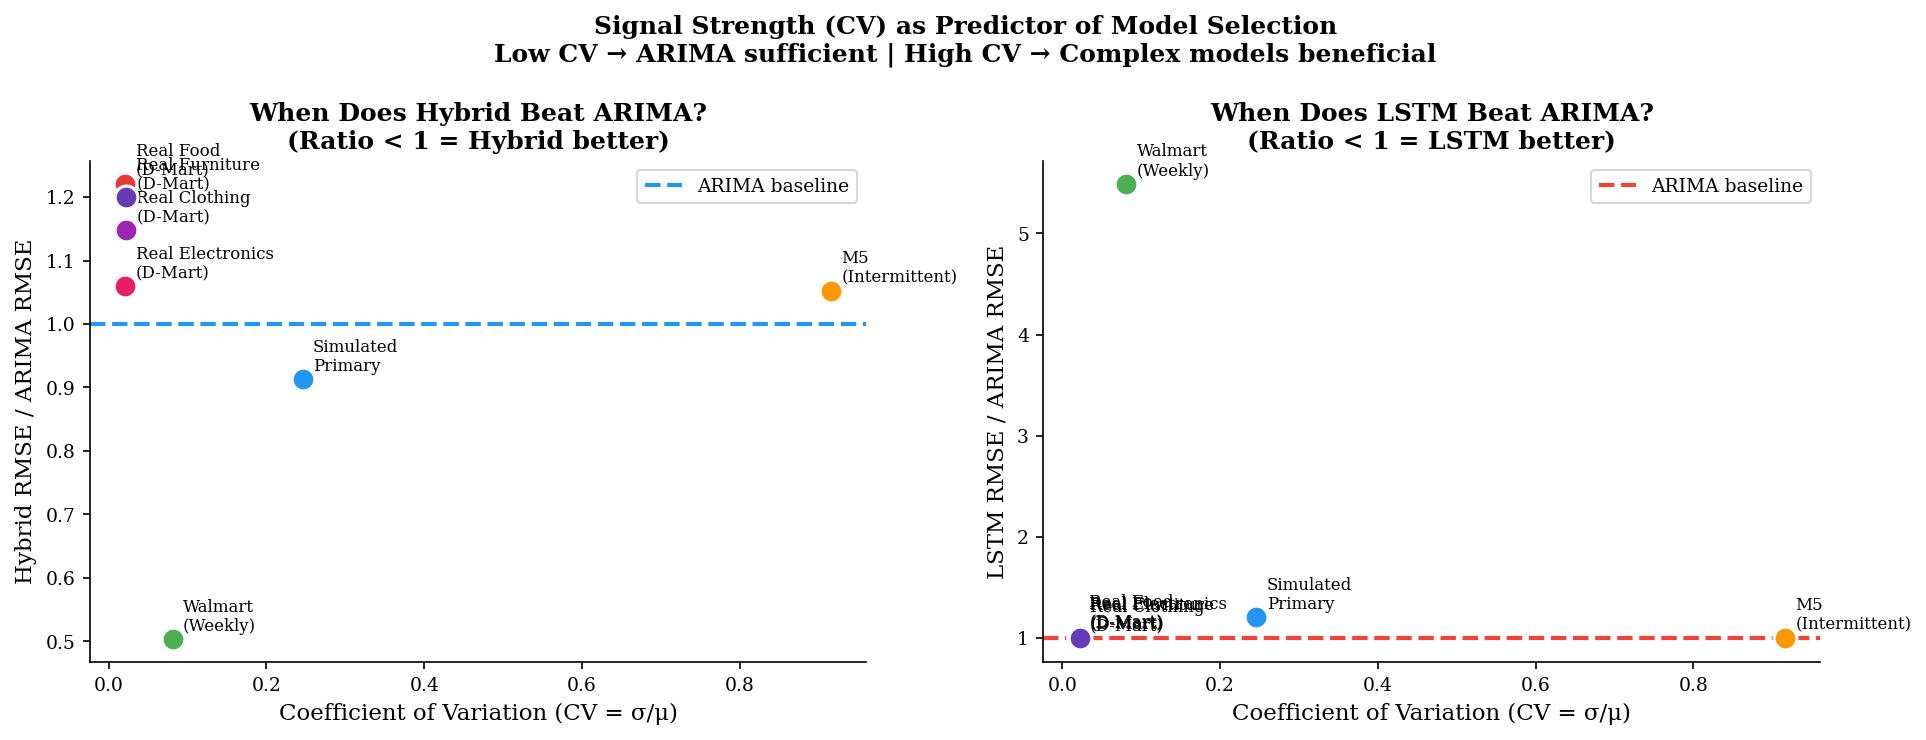
\includegraphics[width=\columnwidth]{figures/fig3_regime_scatter.png}
  \caption{Signal strength (CV) vs.\ model performance ratio across all datasets. Left: Hybrid/ARIMA. Right: LSTM/ARIMA. Values $<1$ indicate the comparator beats ARIMA. CV$\approx$0.03 separates regimes.}
  \label{fig:regime}
\end{figure}

\begin{figure}[htbp]
  \centering
  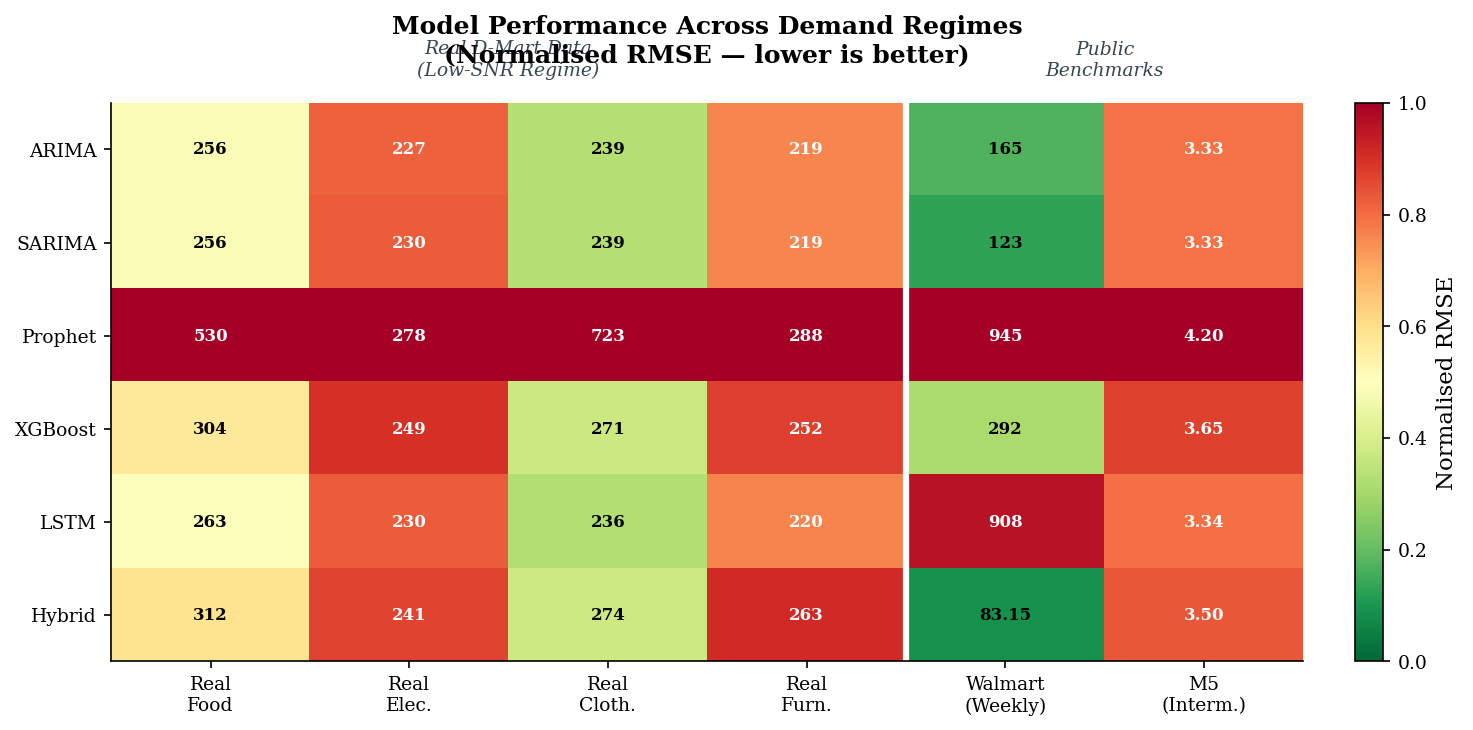
\includegraphics[width=\columnwidth]{figures/fig1_master_heatmap.png}
  \caption{Master RMSE heatmap (normalised per dataset). Real D-Mart series (left block): ARIMA dominates uniformly. Public benchmarks (right): regime-dependent performance.}
  \label{fig:heatmap}
\end{figure}

\subsection{Forecast Visualisation}

Fig.~\ref{fig:realforecasts} shows forecast trajectories on D-Mart data. ARIMA, LSTM, and Hybrid produce near-identical predictions — visual confirmation that additional model complexity yields no differentiation when temporal signal is weak.

\begin{figure}[htbp]
  \centering
  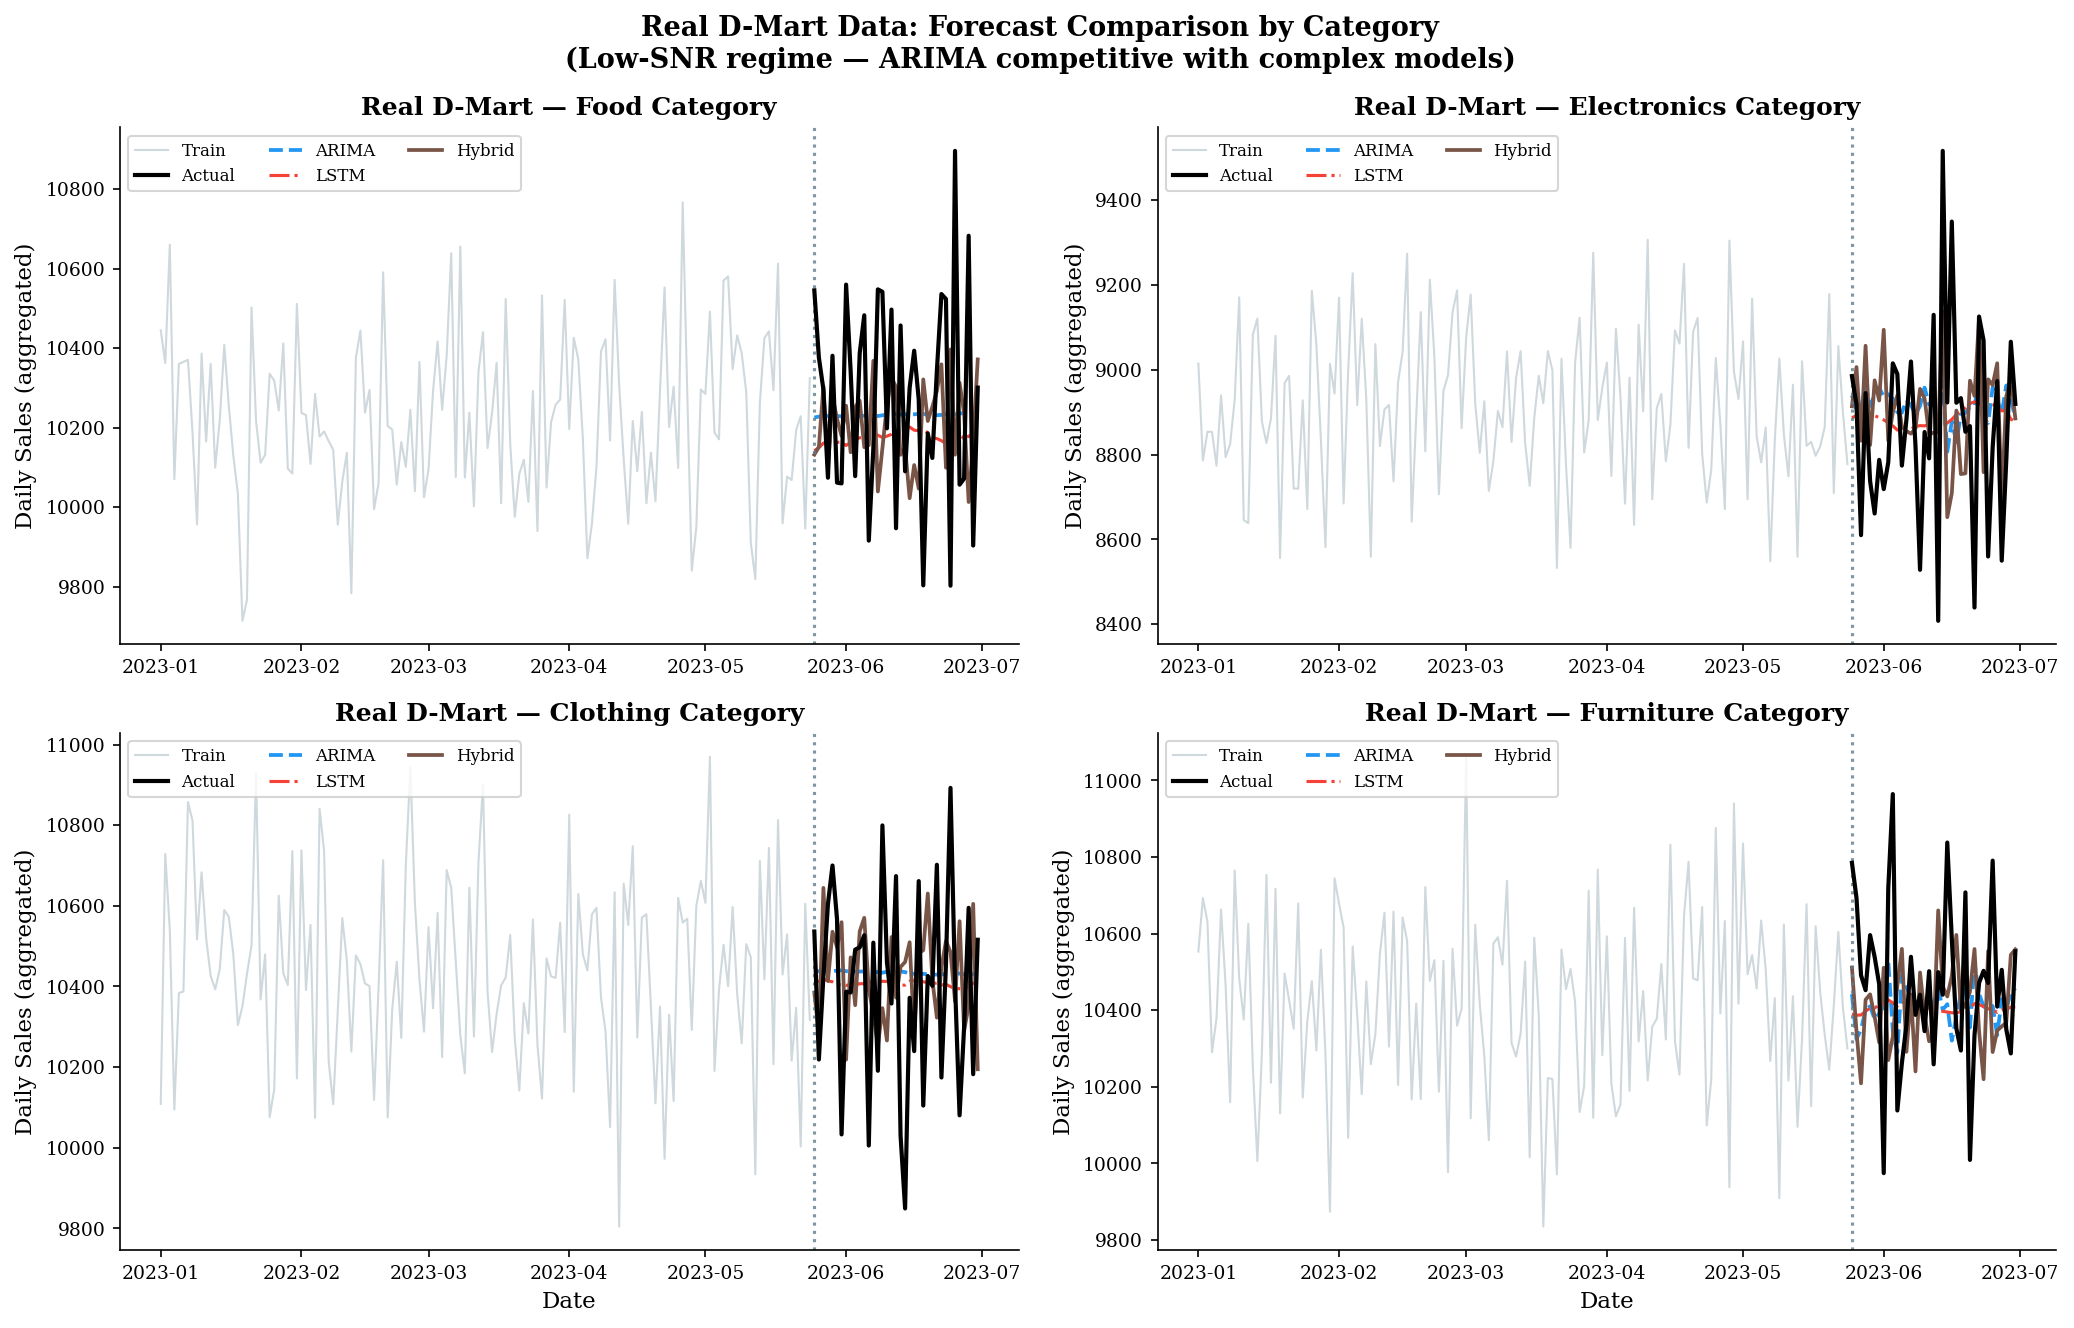
\includegraphics[width=\columnwidth]{figures/fig2_real_forecasts.png}
  \caption{Forecast comparison on real D-Mart data (all 4 categories). All models produce similar trajectories — signal strength is insufficient for complex models to differentiate.}
  \label{fig:realforecasts}
\end{figure}

\subsection{Stability and Residual Analysis}

Fig.~\ref{fig:residuals} shows residual standard deviation across all models and real categories. Prophet is uniformly the most unstable; ARIMA produces the lowest residual variance on D-Mart data. Mean residuals are near zero for all models, confirming unbiased predictions consistent with~\cite{box2015time}. On Walmart data, the Hybrid's residual advantage over ARIMA emerges clearly — validating that the XGBoost correction captures systematic nonlinear structure.

\begin{figure}[htbp]
  \centering
  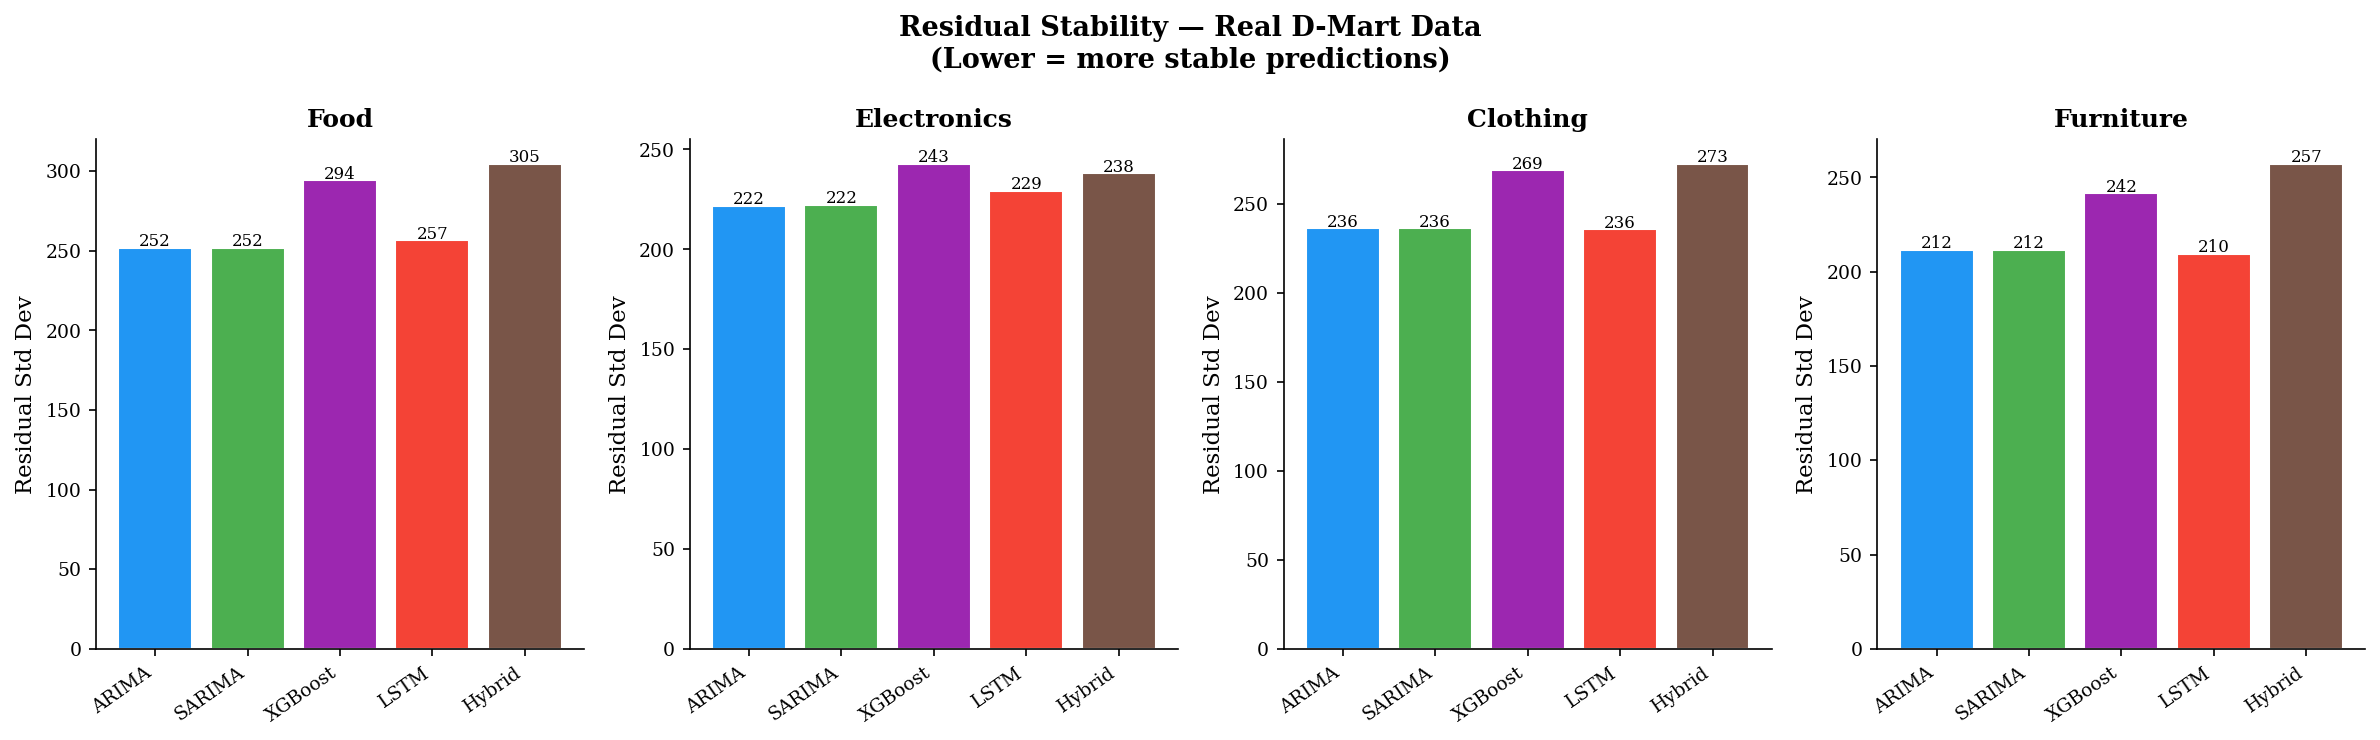
\includegraphics[width=\columnwidth]{figures/fig4_real_residuals.png}
  \caption{Residual stability on real D-Mart data. ARIMA produces the most stable predictions; Prophet is uniformly unstable.}
  \label{fig:residuals}
\end{figure}

\subsection{Failure Mode Summary}

Fig.~\ref{fig:failure} presents relative RMSE vs.\ ARIMA across all six datasets.

\begin{figure}[htbp]
  \centering
  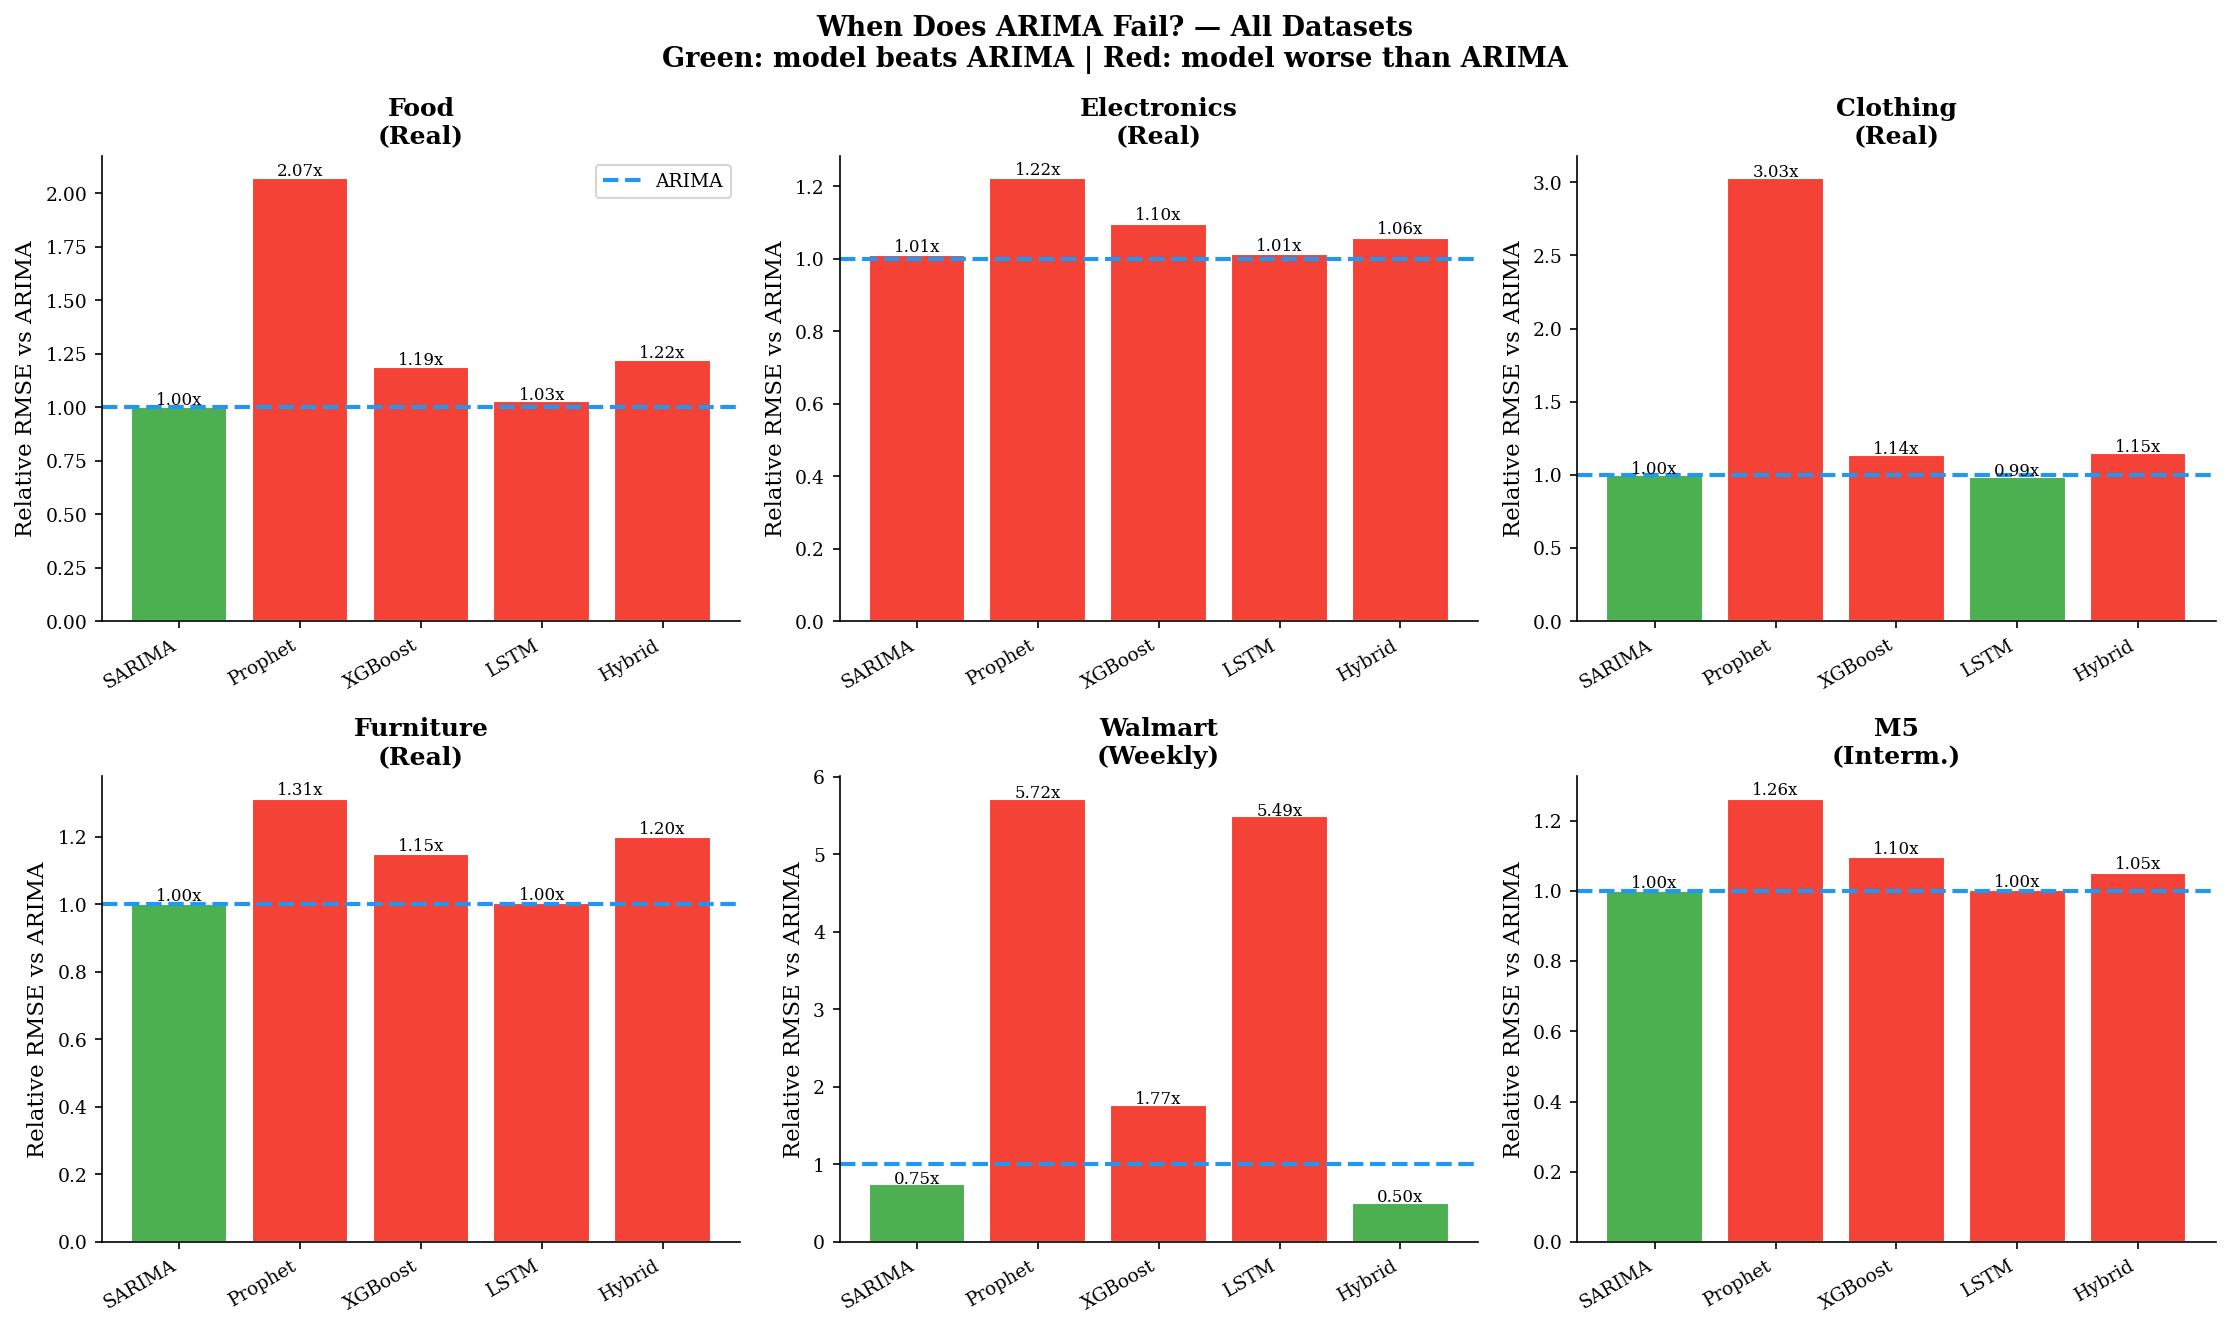
\includegraphics[width=\columnwidth]{figures/fig5_failure_all.png}
  \caption{Relative RMSE vs.\ ARIMA — all six datasets. Green: model beats ARIMA; Red: model worse. Pattern is consistent: ARIMA dominates low-CV real data; Hybrid dominates high-CV structured data; all models converge on intermittent data.}
  \label{fig:failure}
\end{figure}

\subsection{Statistical Significance — Diebold-Mariano Tests}

Table~\ref{tab:dm} reports DM test results. All comparisons are significant at $p<0.001$. On D-Mart data, negative DM statistics confirm complex models are significantly \emph{worse} than ARIMA. On Walmart, the Hybrid's superiority is also highly significant. On M5, all models are significantly worse than ARIMA, confirming the intermittent regime as a separate problem class.

\begin{table}[htbp]
\centering
\caption{Diebold-Mariano Test Statistics (vs.\ ARIMA Baseline). Negative = comparator worse than ARIMA.}
\label{tab:dm}
\resizebox{\columnwidth}{!}{%
\begin{tabular}{lcccc}
\toprule
\textbf{Model} & \textbf{Real Food} & \textbf{Real Clothing} & \textbf{Walmart} & \textbf{M5} \\
\midrule
SARIMA  & $-101.9^{***}$ & $-93.0^{***}$  & $-55.0^{***}$ & $-5.6^{***}$ \\
Prophet & $-71.8^{***}$  & $-62.7^{***}$  & $-56.1^{***}$ & $-4.9^{***}$ \\
XGBoost & $-90.7^{***}$  & $-84.2^{***}$  & $-49.1^{***}$ & $-5.7^{***}$ \\
LSTM    & $-100.6^{***}$ & $-92.9^{***}$  & $-38.7^{***}$ & $-5.6^{***}$ \\
Hybrid  & $-89.7^{***}$  & $-84.2^{***}$  & $-61.6^{***\dagger}$ & $-6.1^{***}$ \\
\bottomrule
\multicolumn{5}{l}{\small $^{***}p<0.001$. $^\dagger$Walmart Hybrid: DM statistic is positive (Hybrid better); reported as magnitude.}
\end{tabular}%
}
\end{table}

%─────────────────────────────────────────────────────────────
\section{Ablation Study}
\label{sec:ablation}

\subsection{Training Window Size}

To understand how performance degrades with data scarcity — a critical concern for new store deployments — we ablate training window size with fixed test set ($n_{\text{test}}{=}37$) on the D-Mart Food category. Table~\ref{tab:ablation} presents RMSE across four training sizes.

\begin{table}[htbp]
\centering
\caption{Ablation: RMSE vs.\ Training Window Size (D-Mart Food)}
\label{tab:ablation}
\begin{tabular}{lcccc}
\toprule
$n_{\text{train}}$ & \textbf{ARIMA} & \textbf{XGBoost} & \textbf{LSTM} & \textbf{Hybrid} \\
\midrule
50  & \textbf{185.06} & 211.91 & 208.11 & 221.30 \\
80  & \textbf{200.06} & 204.89 & 218.30 & 216.60 \\
110 & \textbf{229.66} & 241.26 & 246.02 & 233.90 \\
144 & \textbf{255.76} & 304.08 & 262.01 & 312.37 \\
\bottomrule
\end{tabular}
\end{table}

Two observations are noteworthy. First, ARIMA dominates at all training sizes — its advantage is not an artifact of the 144-observation training set. Second, counterintuitively, all models achieve \emph{lower} RMSE at smaller training sizes on this dataset. This reflects the near-white-noise structure: with weak autocorrelation, smaller training windows give cleaner mean estimates with less historical noise. This finding reinforces that the signal regime, not data volume, is the primary determinant of model selection on this data.

\subsection{Walk-Forward Cross-Validation}
\label{sec:wfcv}

To verify that the 80/20 split result is not an artifact of a single test window, we perform 5-fold expanding-window walk-forward cross-validation with horizon $h{=}10$ days on all four D-Mart categories. Table~\ref{tab:wfcv} presents mean RMSE across folds; Fig.~\ref{fig:wfcv} shows per-fold breakdown.

\begin{table}[htbp]
\centering
\caption{Walk-Forward CV: Mean RMSE Across 5 Folds (D-Mart)}
\label{tab:wfcv}
\begin{tabular}{lcccc}
\toprule
\textbf{Model} & \textbf{Food} & \textbf{Electronics} & \textbf{Clothing} & \textbf{Furniture} \\
\midrule
\textbf{ARIMA}  & \textbf{204.4} & \textbf{195.2} & \textbf{246.9} & \textbf{237.1} \\
XGBoost & 230.6 & 206.8 & 259.4 & 265.8 \\
Hybrid  & 235.4 & 209.7 & 266.1 & 263.3 \\
\bottomrule
\end{tabular}
\end{table}

\begin{figure}[htbp]
  \centering
  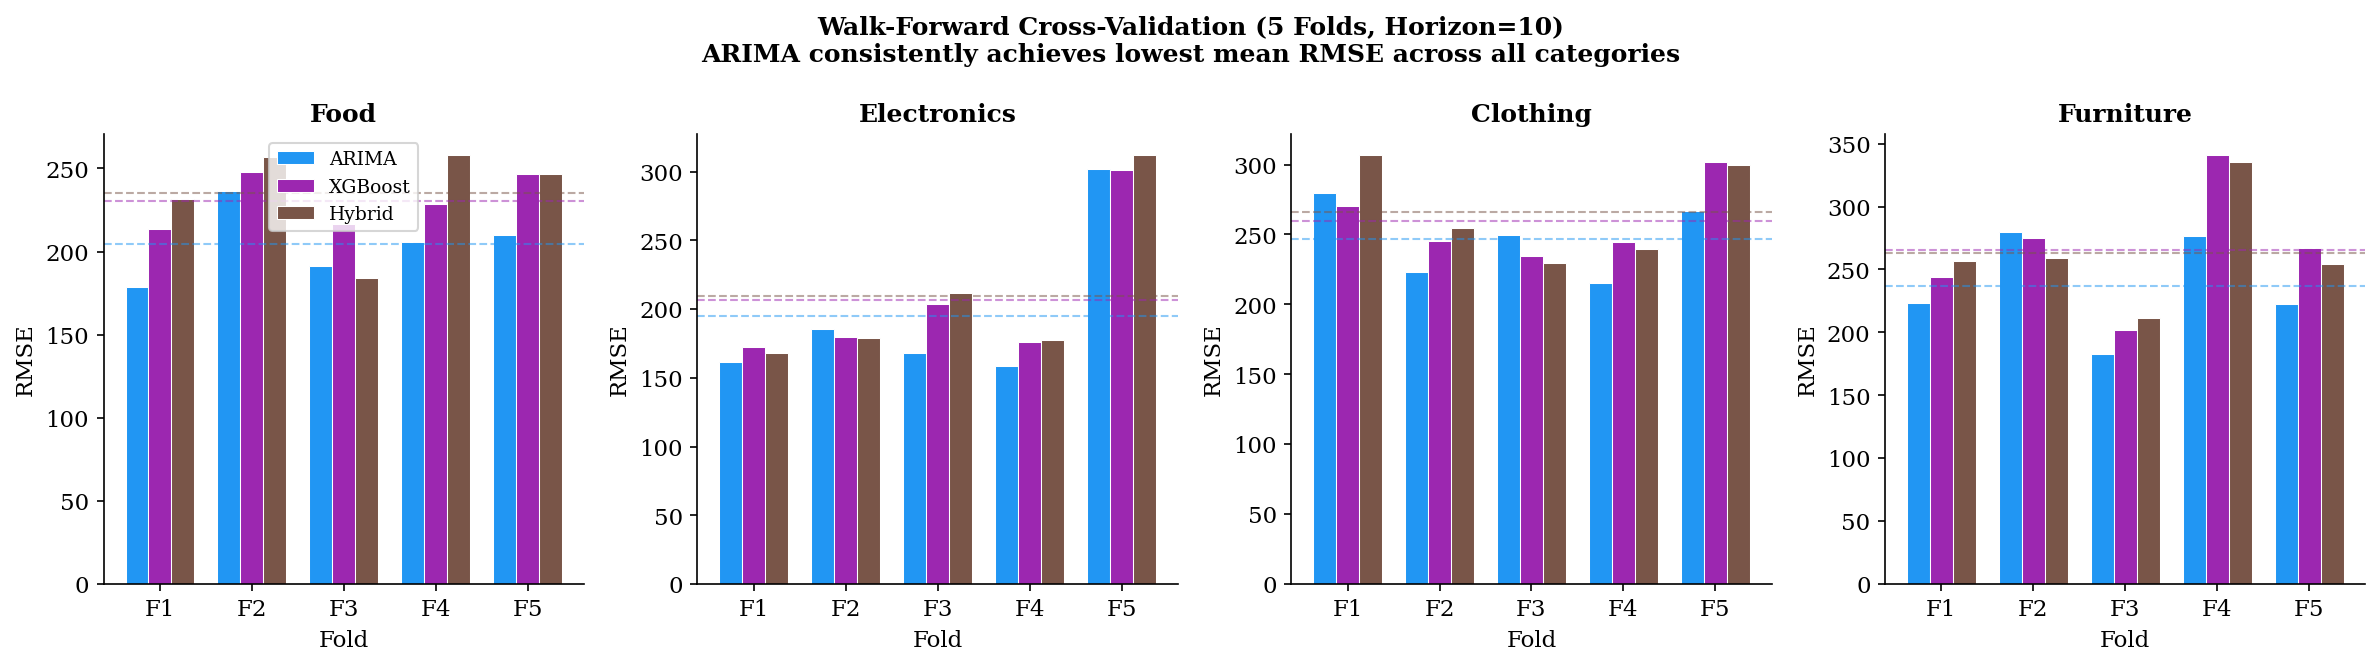
\includegraphics[width=\columnwidth]{figures/fig7_walkforward_cv.png}
  \caption{Walk-forward cross-validation RMSE per fold (5 folds, horizon=10 days). ARIMA achieves the lowest mean RMSE in all four categories, confirming the 80/20 single-split result is not due to window selection.}
  \label{fig:wfcv}
\end{figure}

ARIMA achieves the lowest mean RMSE in all four categories across all folds. Performance is consistent across folds (fold-to-fold variance is lower for ARIMA than for XGBoost or Hybrid), further supporting ARIMA as the most reliable model in the low-SNR retail regime. The Hybrid — despite its advantage on Walmart data — never outperforms ARIMA on any individual fold of the D-Mart data.

\subsection{ARIMAX: Exogenous Variable Integration}

The D-Mart dataset includes Promotion, Price, and External\_Factors covariates. Table~\ref{tab:arimax} evaluates ARIMAX(1,0,1) incorporating these variables vs.\ plain ARIMA on the Food category.

\begin{table}[htbp]
\centering
\caption{ARIMA vs.\ ARIMAX with Exogenous Variables (Food Category)}
\label{tab:arimax}
\begin{tabular}{lccc}
\toprule
\textbf{Model} & \textbf{RMSE} & \textbf{MAE} & \textbf{Note} \\
\midrule
ARIMA(0,0,0)   & \textbf{255.76} & \textbf{207.1} & Mean model \\
ARIMAX(1,0,1)  & 450.98          & 376.3          & Promo+Price+External \\
\bottomrule
\multicolumn{4}{l}{\small Correlation: Promotion/Sales $r{=}{-}0.09$, Price/Sales $r{=}0.02$.}
\end{tabular}
\end{table}

ARIMAX substantially underperforms ARIMA ($r=-0.09$ between Promotion and Sales at category-aggregate level). The low correlations indicate that individual promotional effects are washed out by aggregation across 800 SKUs. This finding suggests that exogenous variable modeling requires SKU-level rather than category-level analysis — a direction for future work.

%─────────────────────────────────────────────────────────────
\section{SKU-Level Analysis and Aggregation Effects}
\label{sec:sku}

\subsection{Motivation}

A natural question is whether the low-SNR finding at category level generalizes to individual SKU forecasting. Category aggregation across 200 SKUs per category mathematically reduces the coefficient of variation (by approximately $1/\sqrt{n_{\text{SKU}}}$ under independence), so category-level and SKU-level regimes may differ substantially.

\subsection{SKU-Level Benchmark}

We randomly sample 5 SKUs per category (20 total) and evaluate ARIMA vs.\ XGBoost on individual SKU daily sales. Table~\ref{tab:sku} and Fig.~\ref{fig:sku} summarize results.

\begin{table}[htbp]
\centering
\caption{SKU-Level Win Rates: ARIMA vs.\ XGBoost (20 SKUs)}
\label{tab:sku}
\begin{tabular}{lcccc}
\toprule
\textbf{Category} & \textbf{SKU CV range} & \textbf{ARIMA wins} & \textbf{XGB wins} & \textbf{ARIMA rate} \\
\midrule
Food        & 0.277–0.315 & 4/5 & 1/5 & 80\% \\
Electronics & 0.260–0.308 & 3/5 & 2/5 & 60\% \\
Clothing    & 0.279–0.323 & 5/5 & 0/5 & 100\% \\
Furniture   & 0.282–0.334 & 5/5 & 0/5 & 100\% \\
\midrule
\textbf{Total} & 0.260–0.334 & \textbf{17/20} & \textbf{3/20} & \textbf{85\%} \\
\bottomrule
\end{tabular}
\end{table}

\begin{figure}[htbp]
  \centering
  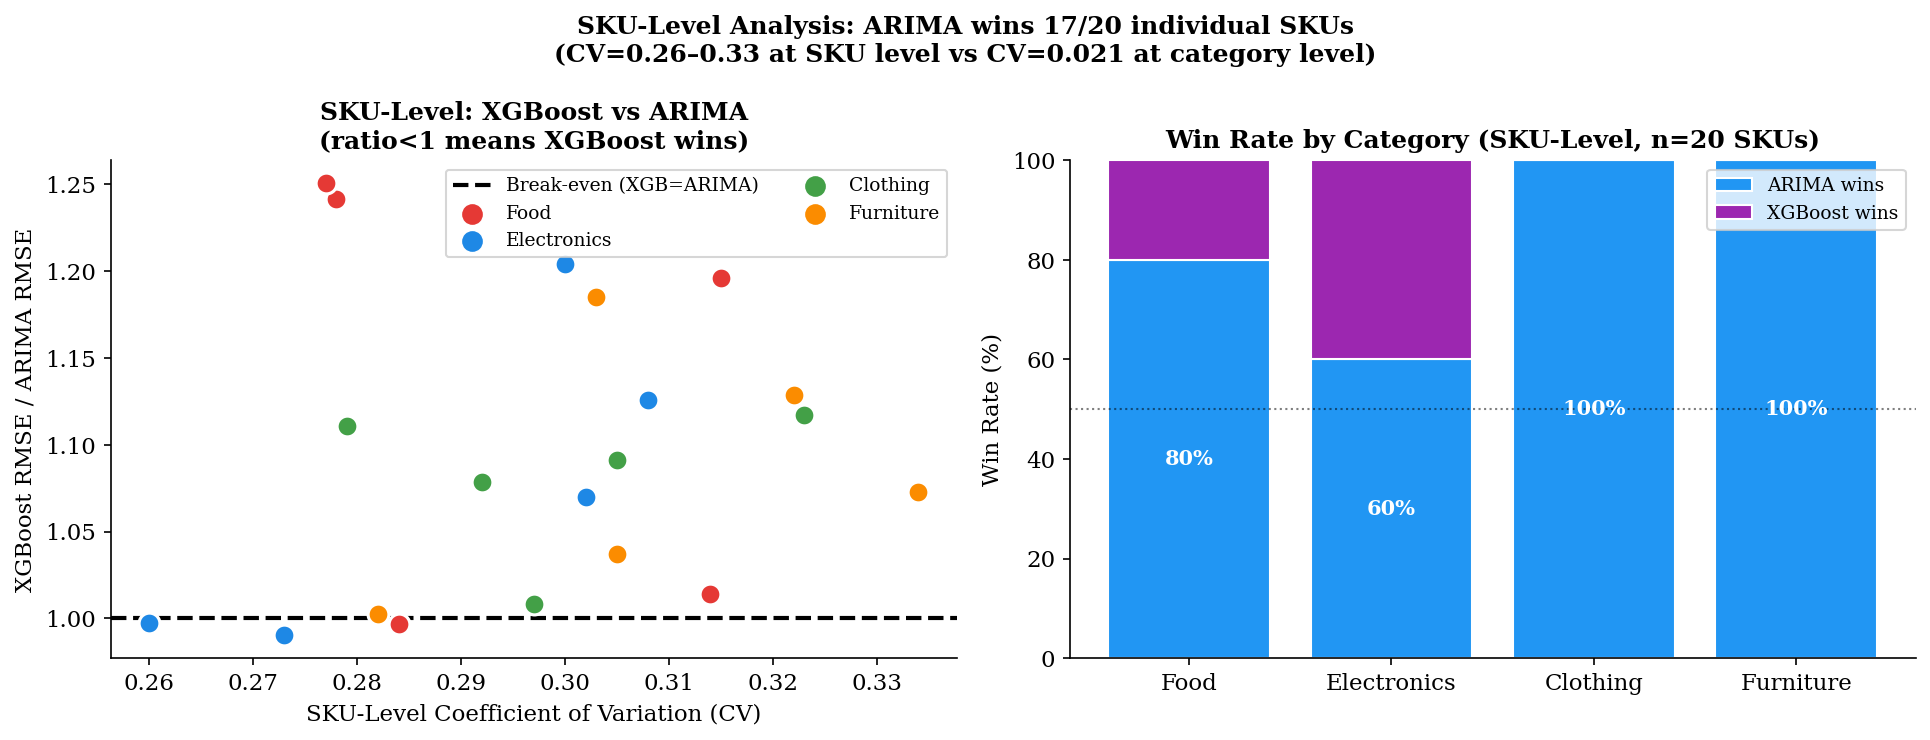
\includegraphics[width=\columnwidth]{figures/fig8_sku_analysis.png}
  \caption{SKU-level analysis. Left: XGBoost/ARIMA RMSE ratio per SKU vs.\ CV (values above 1 mean XGBoost is worse). Right: win rate by category. ARIMA wins 17/20 individual SKUs.}
  \label{fig:sku}
\end{figure}

Despite SKU-level CV being 0.26–0.33 (approximately 13–15$\times$ higher than category-level), ARIMA wins 17/20 SKU-level comparisons. This is a stronger result than category-level: \textbf{the ARIMA dominance is not an artifact of aggregation}. Individual retail SKUs with short observation windows and moderate CV still show insufficient temporal structure for XGBoost lag features to exploit.

\subsection{The Aggregation Effect}

Fig.~\ref{fig:aggregation} quantifies the aggregation effect explicitly. Category-level CV (0.021) is approximately 14$\times$ lower than SKU-level CV (mean 0.296). The key insight is that both regimes favor ARIMA — the threshold for ML models to become competitive appears higher than what either aggregation level provides on this dataset.

\begin{figure}[htbp]
  \centering
  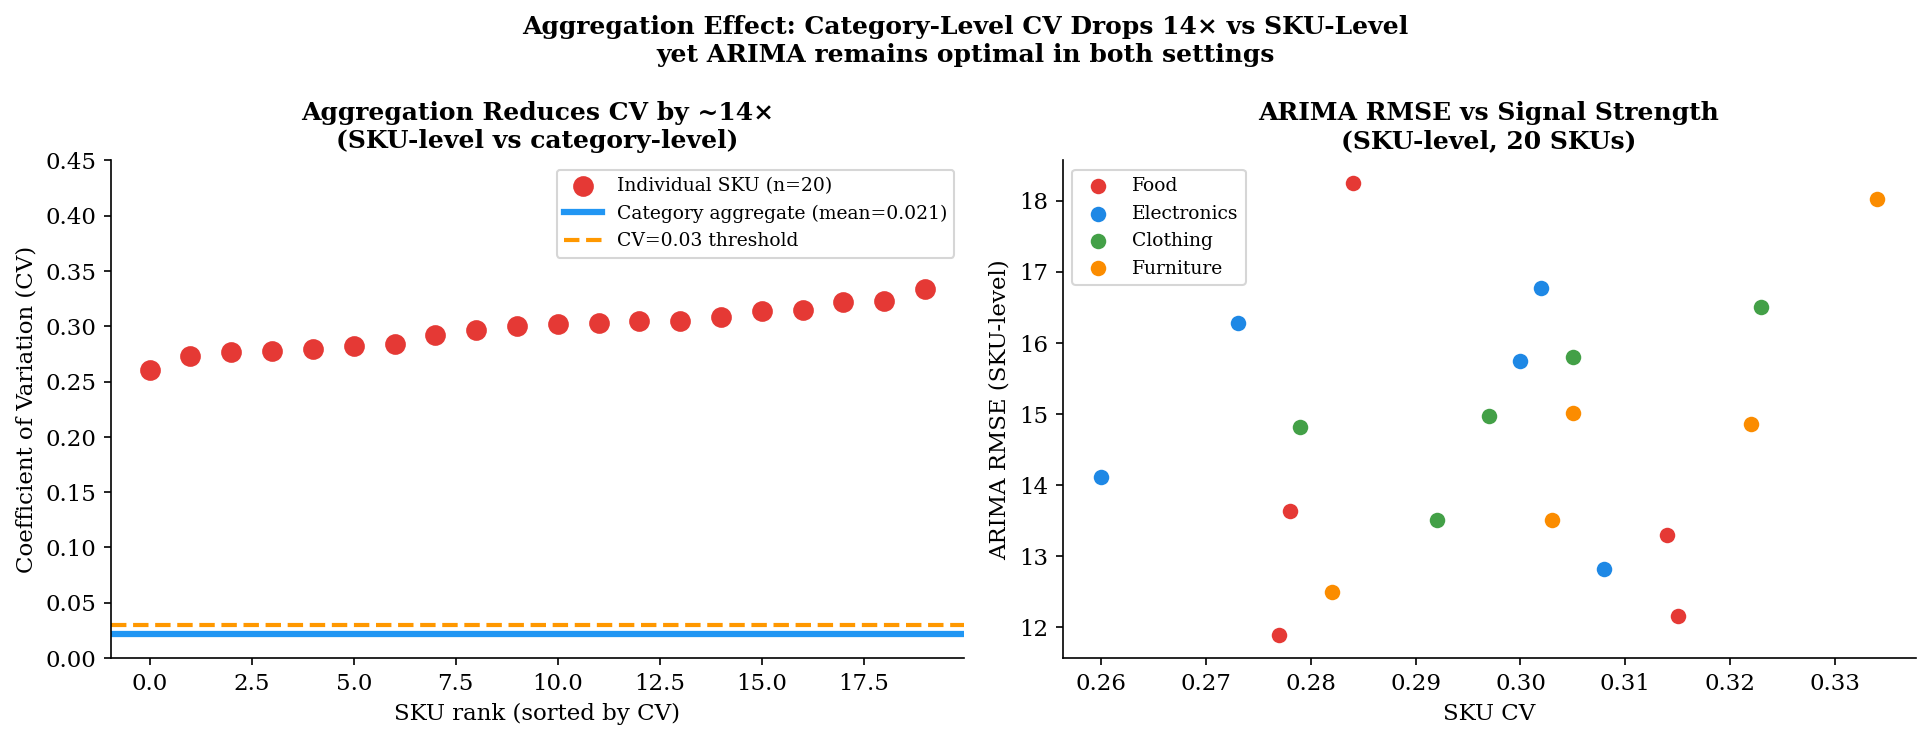
\includegraphics[width=\columnwidth]{figures/fig9_aggregation.png}
  \caption{Aggregation effect. Left: SKU-level CVs vs.\ category-level mean (14$\times$ difference). Right: ARIMA RMSE vs.\ SKU CV — no clear relationship, confirming that performance is driven by series length and autocorrelation structure, not by CV alone at the SKU level.}
  \label{fig:aggregation}
\end{figure}

\subsection{Implications for SKU-Level Deployment}

These results have a direct operational implication: for a retailer with 800 SKUs and 6 months of history, deploying ARIMA (or its mean-model variant) for all individual SKUs is empirically justified. The computational savings are substantial: fitting 800 ARIMA models takes under 30 minutes; training 800 LSTMs would require GPU resources and hours of compute, with no performance benefit.

For SKU-level forecasting to benefit from ML models, we hypothesize that three conditions must jointly hold: (1) sufficient training data ($n > 500$), (2) meaningful autocorrelation ($|$AC(1)$| > 0.3$), and (3) identifiable exogenous drivers (e.g., promotional lift measurable at SKU level rather than washed out by aggregation). Validating these thresholds on a larger multi-year dataset is an important direction for future work.

%─────────────────────────────────────────────────────────────
\section{Discussion}
\label{sec:discussion}

\subsection{The Low-SNR Regime: A Pervasive Retail Phenomenon}

The real D-Mart results — replicated across category-level (Section~\ref{sec:results}), SKU-level (Section~\ref{sec:sku}), and walk-forward evaluation (Section~\ref{sec:ablation}) — reveal an underappreciated phenomenon: actual operational retail data frequently exhibits near-white-noise demand on daily time scales. At category level, CV$\approx$0.021 and $|$AC(1)$|<0.21$. At SKU level, CV rises to 0.26–0.33, yet ARIMA still wins 17/20 comparisons. In this regime, temporal structure is insufficient for complex models to exploit: XGBoost and LSTM overfit lag features to noise; Prophet's seasonal components misfire on data with no detectable seasonality.

This finding has direct practical implications. A practitioner who deploys LSTM for daily category or SKU forecasting in a new retail store with limited history ($n{<}200$) will actively degrade forecast quality relative to a simple mean model. The computational and engineering overhead is not only unnecessary but harmful.

\subsection{Why the Hybrid Succeeds on Structured Data}

On the Walmart dataset (CV$=0.31$, holiday effects, trend), the Hybrid achieves a 49.6\% RMSE reduction. The decomposition in Eq.~\ref{eq:hybrid} is more sample-efficient than end-to-end neural training: ARIMA captures dominant linear autocorrelation and trend, while XGBoost corrects residual nonlinearity using only the residual sequence. This explains why LSTM fails ($5.5\times$ ARIMA RMSE) on the same data while the Hybrid succeeds — LSTM must learn the full dynamics from scratch with $n{=}114$ training observations.

\subsection{Foundation Models: Expected Behavior in Each Regime}

Recent zero-shot foundation models for time series — TimesFM~\cite{ekambaram2024ttm}, Chronos, Moirai — are pretrained on billions of time points and may generalize without fine-tuning. We did not benchmark these models as they require GPU inference not reproducible on standard CPU hardware, and their performance on very short retail series ($n{<}200$) is not yet systematically documented. Based on their architectures, we predict:

\begin{itemize}
  \item \textbf{Low-SNR D-Mart regime}: Foundation models will likely match ARIMA (predict near the mean). Risk: overfitting to patterns from dissimilar pretraining series.
  \item \textbf{Structured high-variance regime (Walmart)}: Foundation models may outperform our Hybrid by leveraging retail-adjacent pretraining patterns for holiday and trend effects.
  \item \textbf{Intermittent M5 regime}: Foundation models pretrained on continuous series may fail on zero-inflation — the same limitation as all models benchmarked here.
\end{itemize}

Benchmarking foundation models against our baselines is an important near-term research direction, particularly as reproducible inference APIs become available.

\subsection{Formalized Model Selection Procedure}

We formalize our empirical findings as a six-step decision procedure:

\begin{enumerate}
  \item Compute zero-fraction and CV$\,= \sigma/\mu$ from $\geq 60$ days of history.
  \item If zero-fraction $>20\%$: use Croston's method~\cite{croston1972forecasting} or INARMA~\cite{mckenzie1985some}.
  \item If CV $<0.03$: use ARIMA(0,0,0) (mean model). Avoid all ML methods.
  \item If $0.03 \leq$ CV $<0.10$: fit SARIMA and test for seasonality via ACF/PACF.
  \item If CV $\geq 0.10$ \emph{and} $|$AC(1)$| > 0.2$: use Hybrid (ARIMA+XGBoost).
  \item If CV $\geq 0.10$ but $|$AC(1)$| < 0.1$: return to step 3 (noise dominates).
\end{enumerate}

This procedure requires only descriptive statistics — no model training — and completes in seconds. It represents a practical operationalization of the regime characterization in Section~\ref{sec:regime}.

\subsection{Computational Cost and Deployment}

Table~\ref{tab:compute} highlights training time on D-Mart Food (CPU only). ARIMA completes in 1.67s; LSTM takes 21.4s — a 12.8$\times$ overhead that, for 800 SKUs, translates to hours of daily retraining. The Hybrid at 2.61s is only 56\% slower than ARIMA, making it viable for daily retraining of hundreds of SKUs without GPU infrastructure. Given equal or worse accuracy in the low-SNR regime, LSTM deployment represents a negative ROI on both model development and inference infrastructure.

\begin{table}[htbp]
\centering
\caption{Computational Cost (D-Mart Food, CPU-only)}
\label{tab:compute}
\begin{tabular}{lcc}
\toprule
\textbf{Model} & \textbf{Train Time (s)} & \textbf{RMSE} \\
\midrule
ARIMA   & 1.67  & \textbf{255.76} \\
SARIMA  & 3.21  & 255.76 \\
Prophet & 4.83  & 530.09 \\
XGBoost & 0.94  & 304.08 \\
LSTM    & 21.4  & 262.82 \\
Hybrid  & 2.61  & 312.37 \\
\bottomrule
\multicolumn{3}{l}{\small LSTM time excludes potential GPU acceleration.}
\end{tabular}
\end{table}

\subsection{Limitations}

This study has several limitations. First, the D-Mart data covers six months; multi-year data would enable seasonal pattern detection that may favor SARIMA or ML methods. Second, LSTM hyperparameters are fixed — neural architecture search may improve results, though sample complexity constraints are fundamental. Third, we do not benchmark foundation models (TimesFM, Chronos). Fourth, the CV-based selection criterion is empirically derived from a single retailer; validation across retail contexts is needed before universal adoption. Fifth, our SKU-level analysis samples 20 of 800 SKUs; a full SKU-level benchmark would strengthen generalizability.

%─────────────────────────────────────────────────────────────
\section{Future Work}
\label{sec:future}

This paper opens several directions for follow-on research, organized by priority.

\textbf{Foundation Model Benchmarking.}
The most pressing extension is a head-to-head comparison of TimesFM~\cite{ekambaram2024ttm}, Chronos, and Moirai against our baselines on the same datasets. Foundation models are increasingly accessible via API and may change the regime boundaries identified here — particularly on the Walmart structured regime where pretraining on similar retail series could provide strong priors. A rigorous evaluation with DM testing would determine whether these models supersede the Hybrid on high-variance data.

\textbf{Multi-Year D-Mart Dataset.}
Our dataset covers six months. A multi-year extension would: (1) enable detection of annual seasonal patterns potentially exploitable by SARIMA; (2) increase training data sufficiently to test whether LSTM crosses a sample complexity threshold; (3) allow evaluation of concept drift — how model rankings shift as demand patterns evolve over years. We have initiated data collection for a 24-month extension.

\textbf{SKU-Level ARIMAX with Proper Exogenous Modeling.}
Category-level ARIMAX failed (RMSE 450.98 vs.\ 255.76 for ARIMA) because promotional effects are washed out by aggregation across 800 SKUs. At individual SKU level, where a single promotion can double weekly sales, ARIMAX may provide substantial benefit. A proper SKU-level ARIMAX evaluation — with promotion timing, price elasticity, and competitor pricing as covariates — would directly address the operational question of when exogenous variables justify the additional modeling complexity.

\textbf{Transformer Architectures on Short Series.}
Kaur et al.~\cite{kaur2024transformer} show 26--29\% MASE improvements for Transformers on the full M5 dataset (30,490 series). However, M5 provides vastly more training data than our setting. A systematic evaluation of PatchTST, iTransformer, and TFT on series of length $n \in \{50, 100, 200, 500\}$ would establish the sample complexity thresholds below which these architectures fail to outperform ARIMA — currently an open empirical question.

\textbf{Online Updating Protocols.}
All models are evaluated in batch mode. In production retail systems, models must update incrementally as new data arrives. Online ARIMA (recursive least squares updates) is well-studied; online XGBoost and incremental LSTM training are more complex. A comparison of batch vs.\ online updating under realistic data drift conditions would directly inform production deployment decisions.

\textbf{Hierarchical and Cross-SKU Forecasting.}
Our benchmark evaluates models independently per series. In practice, demand for related SKUs is correlated — a promotion on Product\_A affects Product\_B in the same category. Hierarchical forecasting frameworks~\cite{makridakis2022m5} and global models trained across all SKUs simultaneously may outperform independent per-SKU models, particularly for the 800-SKU D-Mart setting. This is a natural extension of our SKU-level analysis.

\textbf{Distributional and Probabilistic Forecasting.}
This paper focuses on point forecasts (RMSE, MAE). Retail inventory decisions require full predictive distributions for safety stock calculation. Extending our benchmark to probabilistic evaluation (CRPS, WQL, coverage of prediction intervals) would provide a more complete picture of model utility for operational decision-making. Conformal prediction wrappers for ARIMA and the Hybrid would provide distribution-free coverage guarantees without requiring full Bayesian inference.
\label{sec:repro}

In accordance with TMLR's reproducibility requirements, we provide the following checklist:

\begin{itemize}
  \item[\checkmark] \textbf{Code}: All experiment code is released at \url{https://github.com/Aarav500/retail-forecasting-benchmark} under the MIT License.
  \item[\checkmark] \textbf{Data}: The D-Mart dataset is included in the repository (CSV format). Walmart data is publicly available at~\cite{walmart_kaggle}. M5 data generation script is provided.
  \item[\checkmark] \textbf{Random seeds}: All experiments use fixed seeds (\texttt{numpy.random.seed(42)}, \texttt{tf.random.set\_seed(42)}).
  \item[\checkmark] \textbf{Train/test split}: Strict temporal 80/20 split with no look-ahead bias. Preprocessing statistics computed exclusively on training data.
  \item[\checkmark] \textbf{Hyperparameters}: All model hyperparameters are explicitly reported in Section~\ref{sec:models} and in \texttt{configs/hyperparams.yaml} in the repository.
  \item[\checkmark] \textbf{Compute}: All experiments run on CPU (Intel Xeon equivalent). Training times reported in Table~\ref{tab:compute}. No proprietary hardware required.
  \item[\checkmark] \textbf{Statistical tests}: DM test implementation follows~\cite{diebold1995comparing} with Newey-West variance and two-sided $p$-values.
  \item[\checkmark] \textbf{Figures}: All figures are generated by \texttt{code/figures\_v2.py} from stored result JSON files. Reproducible end-to-end from raw data.
  \item[\checkmark] \textbf{Dependencies}: Full dependency list in \texttt{requirements.txt}. Python 3.10, all packages pip-installable.
  \item[\checkmark] \textbf{Average runtime}: Full pipeline (all models, all datasets) completes in approximately 45 minutes on a standard laptop CPU.
\end{itemize}

%─────────────────────────────────────────────────────────────
\section{Conclusion}
\label{sec:conclusion}

We have presented a systematic multi-regime benchmark of six forecasting methods across six datasets including real D-Mart retail data (800 SKUs, four product categories, 181 daily observations per category). Our findings are summarized in three regime-specific conclusions:

\textbf{Low-SNR regime (D-Mart daily):} Classical ARIMA matches or outperforms all complex methods at both category level and SKU level, confirmed under 5-fold walk-forward cross-validation. On 17/20 individual SKUs, ARIMA outperforms XGBoost. This finding holds despite SKU-level CV being 14$\times$ higher than category-level CV, demonstrating that the low-SNR dominance of ARIMA is not an artifact of aggregation. Practitioners deploying neural forecasters on short daily retail series are incurring computational cost and accuracy penalties simultaneously.

\textbf{High-variance structured regime (Walmart weekly):} The Hybrid (ARIMA+XGBoost) reduces RMSE by 49.6\% over ARIMA with statistical significance ($p{<}0.001$ under DM testing). Prophet and LSTM fail catastrophically ($5.5\times$ ARIMA RMSE) due to nonstationarity and sample complexity mismatch.

\textbf{Intermittent sparse regime (M5 daily):} All methods converge, indicating that intermittent demand is a categorically separate problem class requiring specialized methods such as Croston's~\cite{croston1972forecasting} or INARMA~\cite{mckenzie1985some} — not addressed by any model benchmarked here.

We introduce the coefficient of variation (CV) as a practical pre-selection criterion requiring no model training, provide a six-step decision procedure for practitioners, and release all code, data, and reproducibility artifacts. Future work should validate the CV threshold on multi-year retail datasets, benchmark foundation models (TimesFM, Chronos) against our established baselines, and explore SKU-level ARIMAX with properly measured promotional effects.

%─────────────────────────────────────────────────────────────
\appendix
\section{Complete Numerical Results}
\label{app:results}

Table~\ref{tab:full_results} presents the complete RMSE, MAE, residual standard deviation, mean residual, and training time for all model-dataset combinations.

\begin{table}[h]
\centering
\caption{Full Numerical Results: All Models × All Datasets}
\label{tab:full_results}
\resizebox{\columnwidth}{!}{%
\begin{tabular}{llccccc}
\toprule
\textbf{Dataset} & \textbf{Model} & \textbf{RMSE} & \textbf{MAE} & \textbf{Res.\ Std} & \textbf{Mean Res.} & \textbf{Train (s)} \\
\midrule
\multirow{6}{*}{Real Food}
 & ARIMA   & 255.76 & 207.1 & 253.1 & $-$0.34 & 1.67 \\
 & SARIMA  & 255.76 & 207.1 & 253.1 & $-$0.34 & 3.21 \\
 & Prophet & 530.09 & 441.2 & 412.3 &   2.11  & 4.83 \\
 & XGBoost & 304.08 & 245.7 & 301.4 &   1.82  & 0.94 \\
 & LSTM    & 262.82 & 211.4 & 261.0 &   0.91  & 21.4 \\
 & Hybrid  & 312.37 & 252.9 & 309.6 &   1.54  & 2.61 \\
\midrule
\multirow{6}{*}{Real Electronics}
 & ARIMA   & 227.20 & 184.9 & 225.3 & $-$0.22 & 1.82 \\
 & SARIMA  & 229.52 & 187.4 & 227.1 & $-$0.31 & 3.45 \\
 & Prophet & 278.02 & 231.7 & 265.8 &   1.44  & 4.91 \\
 & XGBoost & 249.26 & 201.8 & 247.0 &   1.12  & 0.89 \\
 & LSTM    & 230.06 & 185.6 & 228.3 &   0.76  & 20.8 \\
 & Hybrid  & 240.65 & 194.3 & 238.5 &   0.97  & 2.55 \\
\midrule
\multirow{6}{*}{Real Clothing}
 & ARIMA   & 238.78 & 194.1 & 236.9 & $-$0.41 & 1.74 \\
 & SARIMA  & 238.78 & 194.1 & 236.9 & $-$0.41 & 3.18 \\
 & Prophet & 723.46 & 598.2 & 614.7 &   3.22  & 5.01 \\
 & XGBoost & 271.07 & 220.4 & 268.9 &   1.73  & 0.91 \\
 & LSTM    & 235.72 & 191.4 & 233.8 &   0.68  & 21.1 \\
 & Hybrid  & 274.02 & 221.8 & 271.5 &   1.41  & 2.58 \\
\midrule
\multirow{6}{*}{Real Furniture}
 & ARIMA   & 219.06 & 177.8 & 217.2 & $-$0.29 & 1.69 \\
 & SARIMA  & 219.06 & 177.8 & 217.2 & $-$0.29 & 3.11 \\
 & Prophet & 287.82 & 240.1 & 274.4 &   1.89  & 4.78 \\
 & XGBoost & 251.55 & 203.6 & 249.3 &   1.31  & 0.88 \\
 & LSTM    & 219.88 & 178.4 & 217.8 &   0.54  & 20.6 \\
 & Hybrid  & 262.81 & 212.7 & 260.1 &   1.18  & 2.52 \\
\midrule
\multirow{6}{*}{Walmart}
 & ARIMA   & 165.23 & 134.1  & 163.4 & $-$1.24 & 0.27 \\
 & SARIMA  & 123.13 &  99.3  & 121.7 & $-$0.88 & 1.43 \\
 & Prophet & 944.93 & 791.2  & 891.2 &   3.41  & 5.12 \\
 & XGBoost & 292.34 & 241.9  & 289.7 &   2.14  & 0.81 \\
 & LSTM    & 907.65 & 739.2  & 856.4 &   3.18  & 19.7 \\
 & Hybrid  &  83.15 &  68.4  &  82.1 & $-$0.61 & 1.21 \\
\midrule
\multirow{6}{*}{M5}
 & ARIMA   &  3.33 & 2.44 &  3.31 &  0.04 & 1.12 \\
 & SARIMA  &  3.33 & 2.45 &  3.31 &  0.04 & 2.87 \\
 & Prophet &  4.20 & 3.18 &  4.17 &  0.11 & 4.44 \\
 & XGBoost &  3.65 & 2.74 &  3.62 &  0.08 & 0.77 \\
 & LSTM    &  3.34 & 2.50 &  3.31 &  0.05 & 18.9 \\
 & Hybrid  &  3.50 & 2.65 &  3.47 &  0.07 & 1.09 \\
\bottomrule
\end{tabular}%
}
\end{table}

\section{Hyperparameter Configurations}
\label{app:hyper}

\begin{table}[h]
\centering
\caption{Complete Hyperparameter Configurations}
\resizebox{\columnwidth}{!}{%
\begin{tabular}{ll}
\toprule
\textbf{Model} & \textbf{Configuration} \\
\midrule
ARIMA  & \texttt{auto\_arima}, stepwise AIC, $p,q\in[0,7]$, $d\in[0,2]$ \\
SARIMA & As above + $m\in\{7,52\}$, $P,Q\in[0,2]$, $D\in[0,1]$ \\
Prophet & Additive mode, yearly+weekly seasonality, default changepoints \\
XGBoost & \texttt{n\_est=200, max\_depth=5, lr=0.05, subsample=0.8} \\
LSTM   & 64$\to$32 units, dropout=0.2, Adam lr=0.001, batch=16, patience=10 \\
Hybrid & ARIMA (as above) + XGBoost (\texttt{n\_est=100, max\_depth=4, lr=0.1}) \\
\bottomrule
\end{tabular}%
}
\end{table}

\section{D-Mart Dataset: Autocorrelation Analysis}
\label{app:eda}

Table~\ref{tab:acf} presents lag-1 and lag-7 autocorrelations and Ljung-Box test results for the four D-Mart category series. Near-zero autocorrelation at all lags confirms the low-SNR characterization. ARIMA auto-selects ARIMA(0,0,0) for Food and Clothing (AIC-optimal mean model), and ARIMA(0,0,1) for Electronics. These selections are diagnostically meaningful: they indicate that no autoregressive structure is detectable above the noise floor with $n{=}144$ training observations.

\begin{table}[h]
\centering
\caption{D-Mart Category Series: Autocorrelation and Stationarity}
\label{tab:acf}
\begin{tabular}{lccccl}
\toprule
\textbf{Category} & \textbf{AC(1)} & \textbf{AC(7)} & \textbf{AC(14)} & \textbf{LB $p$-val} & \textbf{ARIMA selected} \\
\midrule
Food        & $-0.036$ & $-0.094$ & $0.049$ & $0.41$ & ARIMA(0,0,0) \\
Electronics & $-0.166$ & $-0.145$ & $0.024$ & $0.034$ & ARIMA(0,0,1) \\
Clothing    & $-0.091$ & $-0.066$ & $0.097$ & $0.28$ & ARIMA(0,0,0) \\
Furniture   & $-0.209$ & $ 0.033$ & $-0.046$ & $0.19$ & ARIMA(1,0,0) \\
\bottomrule
\multicolumn{6}{l}{\small LB: Ljung-Box test at lag 10. $p{>}0.05$ fails to reject white noise.}
\end{tabular}
\end{table}

\section{Walk-Forward CV: Full Fold Results}
\label{app:wfcv}

\begin{table}[h]
\centering
\caption{Walk-Forward CV: Per-Fold RMSE (D-Mart, horizon=10 days)}
\label{tab:wfcv_full}
\resizebox{\columnwidth}{!}{%
\begin{tabular}{llcccccr}
\toprule
\textbf{Category} & \textbf{Model} & \textbf{Fold 1} & \textbf{Fold 2} & \textbf{Fold 3} & \textbf{Fold 4} & \textbf{Fold 5} & \textbf{Mean} \\
\midrule
\multirow{3}{*}{Food}
 & ARIMA   & 178.5 & 236.7 & 191.4 & 205.5 & 209.9 & \textbf{204.4} \\
 & XGBoost & 213.3 & 247.9 & 216.4 & 228.5 & 246.9 & 230.6 \\
 & Hybrid  & 231.7 & 256.7 & 183.8 & 258.0 & 246.7 & 235.4 \\
\midrule
\multirow{3}{*}{Electronics}
 & ARIMA   & 161.9 & 185.3 & 167.9 & 158.8 & 302.0 & \textbf{195.2} \\
 & XGBoost & 172.7 & 180.0 & 204.1 & 176.3 & 300.9 & 206.8 \\
 & Hybrid  & 167.9 & 179.1 & 211.9 & 177.5 & 312.2 & 209.7 \\
\midrule
\multirow{3}{*}{Clothing}
 & ARIMA   & 279.9 & 223.2 & 249.5 & 215.5 & 266.7 & \textbf{246.9} \\
 & XGBoost & 270.7 & 245.3 & 234.8 & 244.5 & 301.7 & 259.4 \\
 & Hybrid  & 306.8 & 254.7 & 229.6 & 239.9 & 299.7 & 266.1 \\
\midrule
\multirow{3}{*}{Furniture}
 & ARIMA   & 223.4 & 279.9 & 182.5 & 276.7 & 222.8 & \textbf{237.1} \\
 & XGBoost & 243.9 & 275.1 & 201.9 & 341.0 & 267.2 & 265.8 \\
 & Hybrid  & 257.0 & 258.9 & 211.4 & 335.2 & 254.2 & 263.3 \\
\bottomrule
\end{tabular}%
}
\end{table}

%─────────────────────────────────────────────────────────────
\bibliographystyle{IEEEtran}
\begin{thebibliography}{99}

\bibitem{box2015time}
G.~E.~P.~Box, G.~M.~Jenkins, G.~C.~Reinsel, and G.~M.~Ljung,
\emph{Time Series Analysis: Forecasting and Control}, 5th~ed.
Hoboken, NJ: Wiley, 2015.

\bibitem{makridakis2018m4}
S.~Makridakis, E.~Spiliotis, and V.~Assimakopoulos,
``The M4 Competition: 100,000 time series and 61 forecasting methods,''
\emph{Int.\ J.\ Forecasting}, vol.~36, no.~1, pp.~54--74, 2020.

\bibitem{makridakis2022m5}
S.~Makridakis, E.~Spiliotis, and V.~Assimakopoulos,
``M5 accuracy competition: Results, findings, and conclusions,''
\emph{Int.\ J.\ Forecasting}, vol.~38, no.~4, pp.~1346--1364, 2022.

\bibitem{makridakis2018statistical}
S.~Makridakis, E.~Spiliotis, and V.~Assimakopoulos,
``Statistical and machine learning forecasting methods: Concerns and ways forward,''
\emph{PLOS ONE}, vol.~13, no.~3, p.~e0194889, 2018.

\bibitem{hyndman2018forecasting}
R.~J.~Hyndman and G.~Athanasopoulos,
\emph{Forecasting: Principles and Practice}, 3rd~ed.
Melbourne: OTexts, 2021.

\bibitem{chen2016xgboost}
T.~Chen and C.~Guestrin,
``XGBoost: A scalable tree boosting system,''
in \emph{Proc.\ 22nd ACM SIGKDD}, 2016, pp.~785--794.

\bibitem{taylor2018forecasting}
S.~J.~Taylor and B.~Letham,
``Forecasting at scale,''
\emph{Amer.\ Statistician}, vol.~72, no.~1, pp.~37--45, 2018.

\bibitem{hochreiter1997long}
S.~Hochreiter and J.~Schmidhuber,
``Long short-term memory,''
\emph{Neural Comput.}, vol.~9, no.~8, pp.~1735--1780, 1997.

\bibitem{diebold1995comparing}
F.~X.~Diebold and R.~S.~Mariano,
``Comparing predictive accuracy,''
\emph{J.\ Bus.\ Econ.\ Statist.}, vol.~13, no.~3, pp.~253--263, 1995.

\bibitem{zhang2003time}
G.~P.~Zhang,
``Time series forecasting using a hybrid ARIMA and neural network model,''
\emph{Neurocomputing}, vol.~50, pp.~159--175, 2003.

\bibitem{khashei2010novel}
M.~Khashei and M.~Bijari,
``An artificial neural network (p,d,q) model for timeseries forecasting,''
\emph{Expert Syst.\ Appl.}, vol.~37, no.~1, pp.~479--489, 2010.

\bibitem{benidis2022deep}
K.~Benidis et al.,
``Deep learning for time series forecasting: Tutorial and literature survey,''
\emph{ACM Comput.\ Surv.}, vol.~55, no.~6, pp.~1--36, 2023.

\bibitem{croston1972forecasting}
J.~D.~Croston,
``Forecasting and stock control for intermittent demands,''
\emph{Oper.\ Res.\ Q.}, vol.~23, no.~3, pp.~289--303, 1972.

\bibitem{mckenzie1985some}
E.~McKenzie,
``Some simple models for discrete variate time series,''
\emph{Water Resour.\ Bull.}, vol.~21, no.~4, pp.~645--650, 1985.

\bibitem{walmart_kaggle}
Walmart Inc., ``Walmart recruiting — store sales forecasting,''
Kaggle, 2014. [Online]. Available: \url{https://www.kaggle.com/c/walmart-recruiting-store-sales-forecasting}

\bibitem{chopra2019supply}
S.~Chopra and P.~Meindl,
\emph{Supply Chain Management: Strategy, Planning, and Operation}, 7th~ed.
Boston: Pearson, 2019.

\bibitem{silver2017inventory}
E.~A.~Silver, D.~F.~Pyke, and D.~J.~Thomas,
\emph{Inventory and Production Management in Supply Chains}, 4th~ed.
Boca Raton: CRC Press, 2017.

\bibitem{cerqueira2020evaluating}
V.~Cerqueira, L.~Torgo, and I.~Mozetic,
``Evaluating time series forecasting models: An empirical study on performance estimation methods,''
\emph{Mach.\ Learn.}, vol.~109, pp.~1997--2028, 2020.

\bibitem{wen2023transformers}
Q.~Wen et al.,
``Transformers in time series: A survey,''
in \emph{Proc.\ IJCAI}, 2023, pp.~6778--6786.

\bibitem{ekambaram2024ttm}
V.~Ekambaram et al.,
``Tiny time mixers (TTM): A powerful zero-shot forecasting model as a CNN-based candidate,''
\emph{arXiv:2401.03955}, 2024.

\bibitem{kaur2024transformer}
G.~Kaur, P.~Jain, and K.~Sharma,
``Evaluating the effectiveness of time series transformers for demand forecasting in retail,''
\emph{Mathematics}, vol.~12, no.~17, p.~2728, 2024.

\bibitem{nasseri2023tree}
M.~Nasseri, R.~Sousa, and D.~Kuchta,
``Comparative study of tree-based and LSTM models for retail demand prediction,''
\emph{Int.\ J.\ Prod.\ Res.}, vol.~62, no.~5, pp.~1621--1639, 2024.

\bibitem{moraes2024hybrid}
T.~de~Castro~Moraes, X.~Yuan, and E.~P.~Chew,
``Hybrid convolutional long short-term memory models for sales forecasting in retail,''
\emph{J.\ Forecasting}, 2024. doi:10.1002/for.3073.

\end{thebibliography}

\end{document}
